\documentclass[11pt,a4paper]{article}
\usepackage[T1]{fontenc}
\usepackage[utf8]{inputenc}
\usepackage{lmodern}
\usepackage[margin=2.5cm]{geometry}
\usepackage{xcolor}
\usepackage{booktabs}
\usepackage{enumitem}
\usepackage{parskip}
\usepackage{graphicx}
\usepackage{float}
% Screenshots are in docs/img. Compile from inside docs/.
\graphicspath{{img/}}
\usepackage[colorlinks=true,linkcolor=black,urlcolor=teal]{hyperref}

\definecolor{accent}{HTML}{0E5A45}
\newcommand{\term}[1]{\textbf{\textcolor{accent}{#1}}}
\newcommand{\ui}[1]{\textsf{\textbf{#1}}}
\setlist{itemsep=2pt,topsep=4pt}

\title{\textbf{Community Status Network}\\[4pt]\large A plain-language guide: what it is, how it works, and how to use it}
\author{Marvin Wamoni}
\date{November 2026}

\begin{document}
\maketitle

\section{What is this?}

Imagine a notice board at the centre of a neighbourhood. When the power goes out, a water point
runs dry, or a road is blocked, somebody pins up a note. Everybody who walks past sees it. Later,
a trusted person checks whether the note is true and marks it as confirmed, and when the problem is
fixed they mark it as solved.

The \emph{Community Status Network} is that notice board, on computers and phones. It has one
extra property that an ordinary notice board (and an ordinary website) does not have:

\begin{quote}
\emph{The board is kept on three computers at the same time. If one of them breaks, the board
keeps working and no note is lost.}
\end{quote}

That second part is the reason the project exists. Building a website that stores notes is easy.
Building one that keeps going when a computer dies in the middle of the day is the hard and
interesting part, and it is what this document explains.

\section{Who uses it}

There are three kinds of people:

\begin{description}[leftmargin=2.2cm,style=nextline]
\item[Residents] report problems (``No power on Kimera Road'') and can correct the wording of a
report afterwards.
\item[Moderators] are trusted members of the community. They can do everything a resident can,
and they can also mark a report as \emph{verified} (``yes, this is real'') and \emph{resolved}
(``this is fixed now'').
\item[Viewers] just watch. Their screen updates by itself the moment anything changes; they never
need to press refresh.
\end{description}

Every report is in one of three states: \term{open} (just reported), \term{verified} (a moderator
confirmed it) or \term{resolved} (fixed).

\section{The ideas behind it, without the jargon}

You do not need to be a programmer to follow this section. Each idea is a simple rule.

\subsection{Three copies of everything}

The system runs as three programs, called \term{nodes} and named N1, N2 and N3. Each node holds a
complete copy of every report. You can open the system through any of the three and you will see
the same thing. In a classroom demo the three nodes run on one laptop; in real use they would be
three different machines.

\subsection{One node is in charge of changes}

If three computers each accepted changes on their own, they would quickly disagree with each
other. So at any moment exactly one node is the \term{leader}. Every change (a new report, an
edit) goes through the leader, which decides the order of changes and passes them on to the other
two, called \term{followers}.

You never have to know which node is the leader. If you send a change to a follower, it quietly
hands it to the leader for you and gives you back the leader's answer.

\subsection{Write it down first}

Before a node tells anybody ``your report is saved'', it writes the change into a file on its
disk, one line per change, and makes sure the line has really reached the disk. Think of a
shopkeeper who writes every sale in a notebook \emph{before} handing over the goods. This notebook
is called the \term{write-ahead log}.

The benefit: if a node crashes and is started again, it simply reads its notebook from the first
line to the last and ends up knowing everything it knew before the crash.

\subsection{Two out of three must agree}

When the leader receives a change, it writes it in its own notebook and sends it to both
followers. It only replies ``saved'' once \emph{at least one} follower has also written it down.
So a saved change always exists on at least two of the three computers. This is called a
\term{majority} (two out of three).

This is the rule that makes the promise ``no saved report is ever lost'' true: whichever single
computer dies, at least one other still has the change.

\subsection{Version numbers stop people overwriting each other}

Suppose Alice and Grace both open the same report at the same moment and both start changing it.
Without protection, whoever saves last would silently wipe out the other person's work.

To prevent this, every report carries a \term{version number}. It starts at 1 and goes up by one
with every change. When you save an edit, your screen also tells the system which version you
were looking at. If the report has moved on since then, the system refuses your edit and shows
you what changed. You then decide what to do. Nothing is ever overwritten behind anyone's back.

\subsection{Nodes check on each other}

Once every second, each node sends the others a tiny ``I am alive'' message, called a
\term{heartbeat}. If a node has been silent for three seconds, the others treat it as dead.

If the dead node was the leader, the survivors pick a new one using a simple rule: the living
node with the lowest name wins (N1 before N2 before N3). This takes a little over three seconds.
During those few seconds you can still read everything, but new changes have to wait; the app
waits for you and sends your change as soon as the new leader is ready.

\subsection{Screens update by themselves}

Your browser keeps one connection open to a node, and the node pushes every change down that
connection as it happens. This is the \term{live feed}. If the node you are connected to dies,
your browser connects to another one and asks for ``everything after the last change I saw'', so
you miss nothing.

\section{What happens when you post a report}

\begin{enumerate}
\item You fill in the form and press \ui{Post report}.
\item Your browser sends the report to the node it is connected to.
\item If that node is a follower, it passes the report to the leader.
\item The leader gives the report a number (R1, R2, \dots), writes it in its notebook, and sends
it to both followers.
\item As soon as one follower has written it down too, the leader replies ``saved''.
\item Every node pushes the new report to all the screens connected to it. Everyone sees it
appear, usually within a few thousandths of a second.
\end{enumerate}

\section{What happens when a computer dies}

\begin{description}[style=nextline,leftmargin=0.6cm]
\item[A follower dies.] Almost nothing changes. The leader still has one follower left, so two
out of three can still agree. People connected to the dead node are moved to another one.
\item[The leader dies.] After about three seconds the others notice and choose a new leader.
Changes made during those seconds are retried automatically and go through once the new leader is
ready. Reading is never interrupted.
\item[The dead computer comes back.] It reads its notebook to remember what it knew, asks the
current leader for everything it missed, and rejoins as a follower. It does not take the
leadership back.
\item[Two computers die.] One survivor is not a majority, so it refuses new changes rather than
risk losing them. Reports can still be read. As soon as a second node returns, changes work again.
\end{description}

\section{How to use the system}

\subsection{What you need}

A computer with Python~3 installed. Nothing else: there is nothing to download or install, and no
internet connection is needed.

\subsection{Starting it}

\paragraph{The quick way.} Open a terminal in the project folder and type:
\begin{verbatim}
python3 demo.py
\end{verbatim}
This starts the three nodes and walks through a guided tour: it posts a report, edits it, shows a
rejected conflicting edit, kills the leader, shows the others taking over, and brings the dead
node back. When the tour ends the three nodes keep running. Press Ctrl-C to stop everything. Use
\texttt{python3 demo.py -{}-pause} if you want it to wait for you to press Enter between steps.

\paragraph{By hand.} Open three terminals in the project folder and run one command in each:
\begin{verbatim}
python3 -m csn.server --id N1
python3 -m csn.server --id N2
python3 -m csn.server --id N3
\end{verbatim}

\paragraph{On three separate laptops.} Connect them to the same Wi-Fi or network. Open the file
\texttt{config.json} and replace the addresses with each laptop's network address, for example
\texttt{"N1": "192.168.1.10:8001"}. Copy the project folder (with the edited file) to all three
laptops, then run the matching command from above on each one.

\subsection{Opening the web app}

In a web browser, on a laptop or a phone, go to any one of these addresses:
\begin{verbatim}
http://127.0.0.1:8001/      http://127.0.0.1:8002/      http://127.0.0.1:8003/
\end{verbatim}
(On the three-laptop setup, use the laptop addresses from \texttt{config.json} instead.) All
three show the same reports.

\begin{figure}[H]
\centering
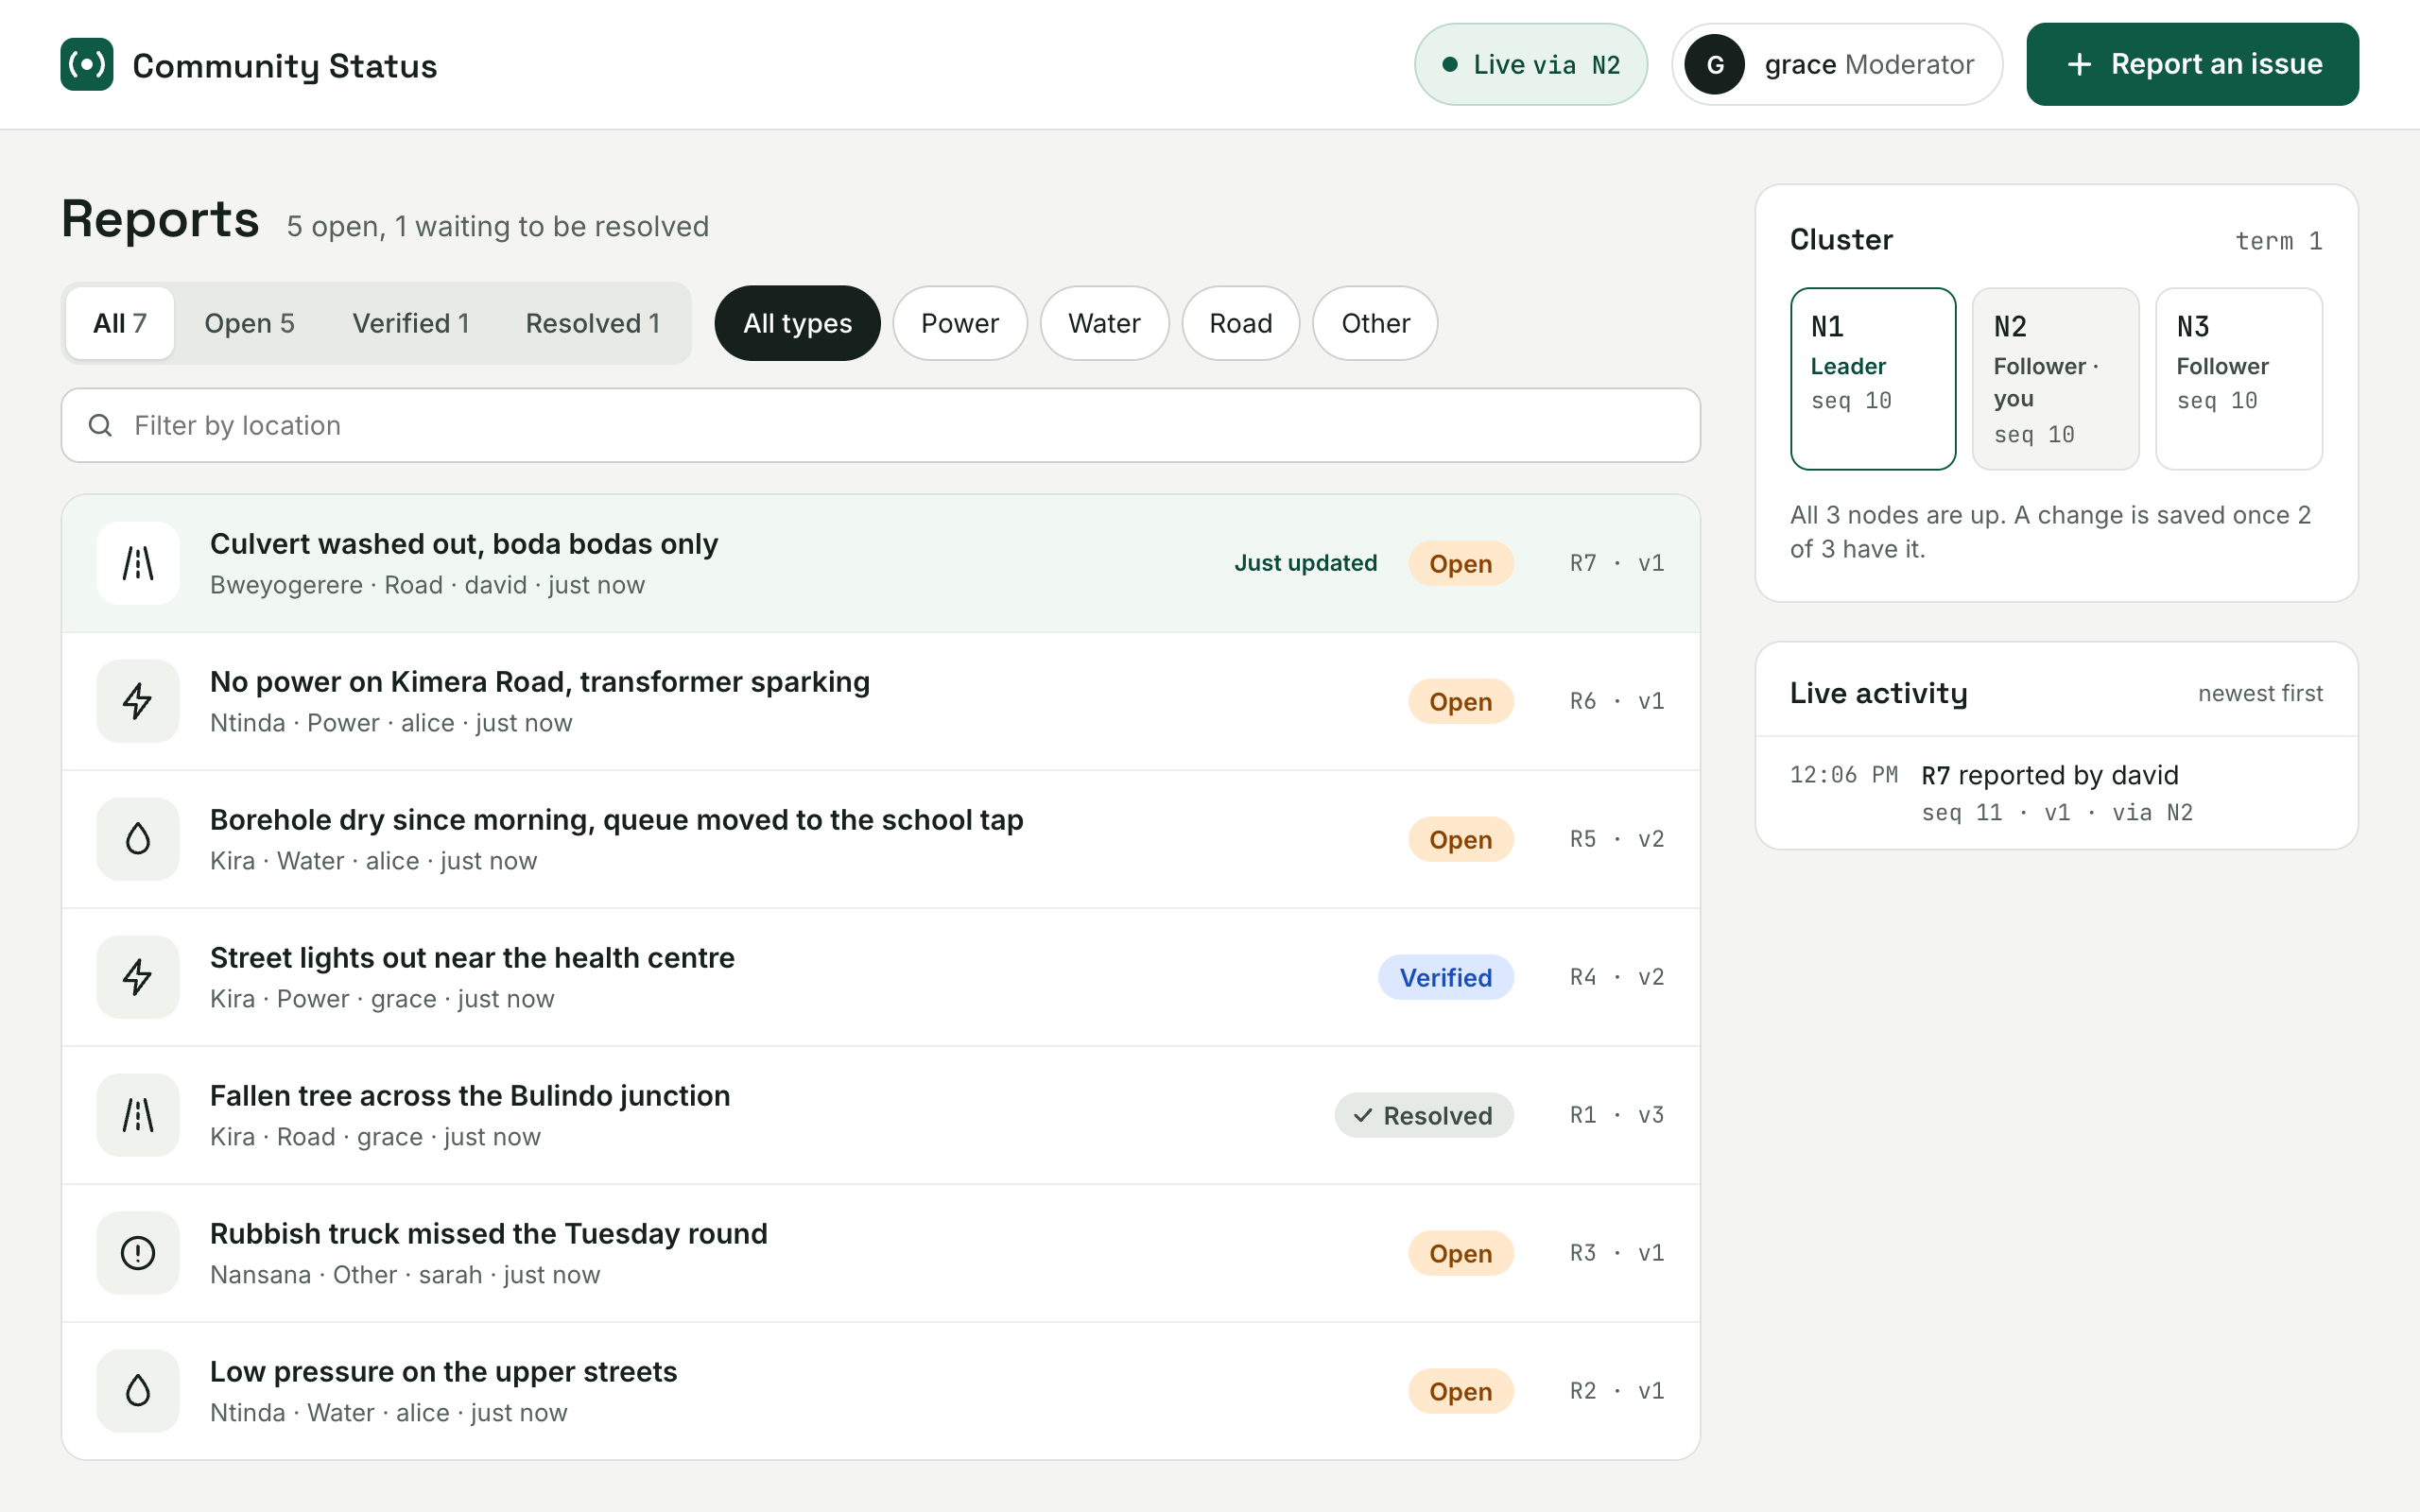
\includegraphics[width=0.95\textwidth]{guide-home.png}
\caption{The main screen. Left: the list of reports with the filters above it. Right: the three nodes and the list of live changes. Top right: the live indicator, your name and role, and the button for reporting a problem.}
\end{figure}

\subsection{Telling it who you are}

Click the round badge at the top right. Type your name and choose \ui{Resident} or
\ui{Moderator}, then press \ui{Save}. The browser remembers this. There are no passwords in this
prototype, so the role is simply the one you choose; see Section~\ref{sec:limits}.

\begin{figure}[H]
\centering
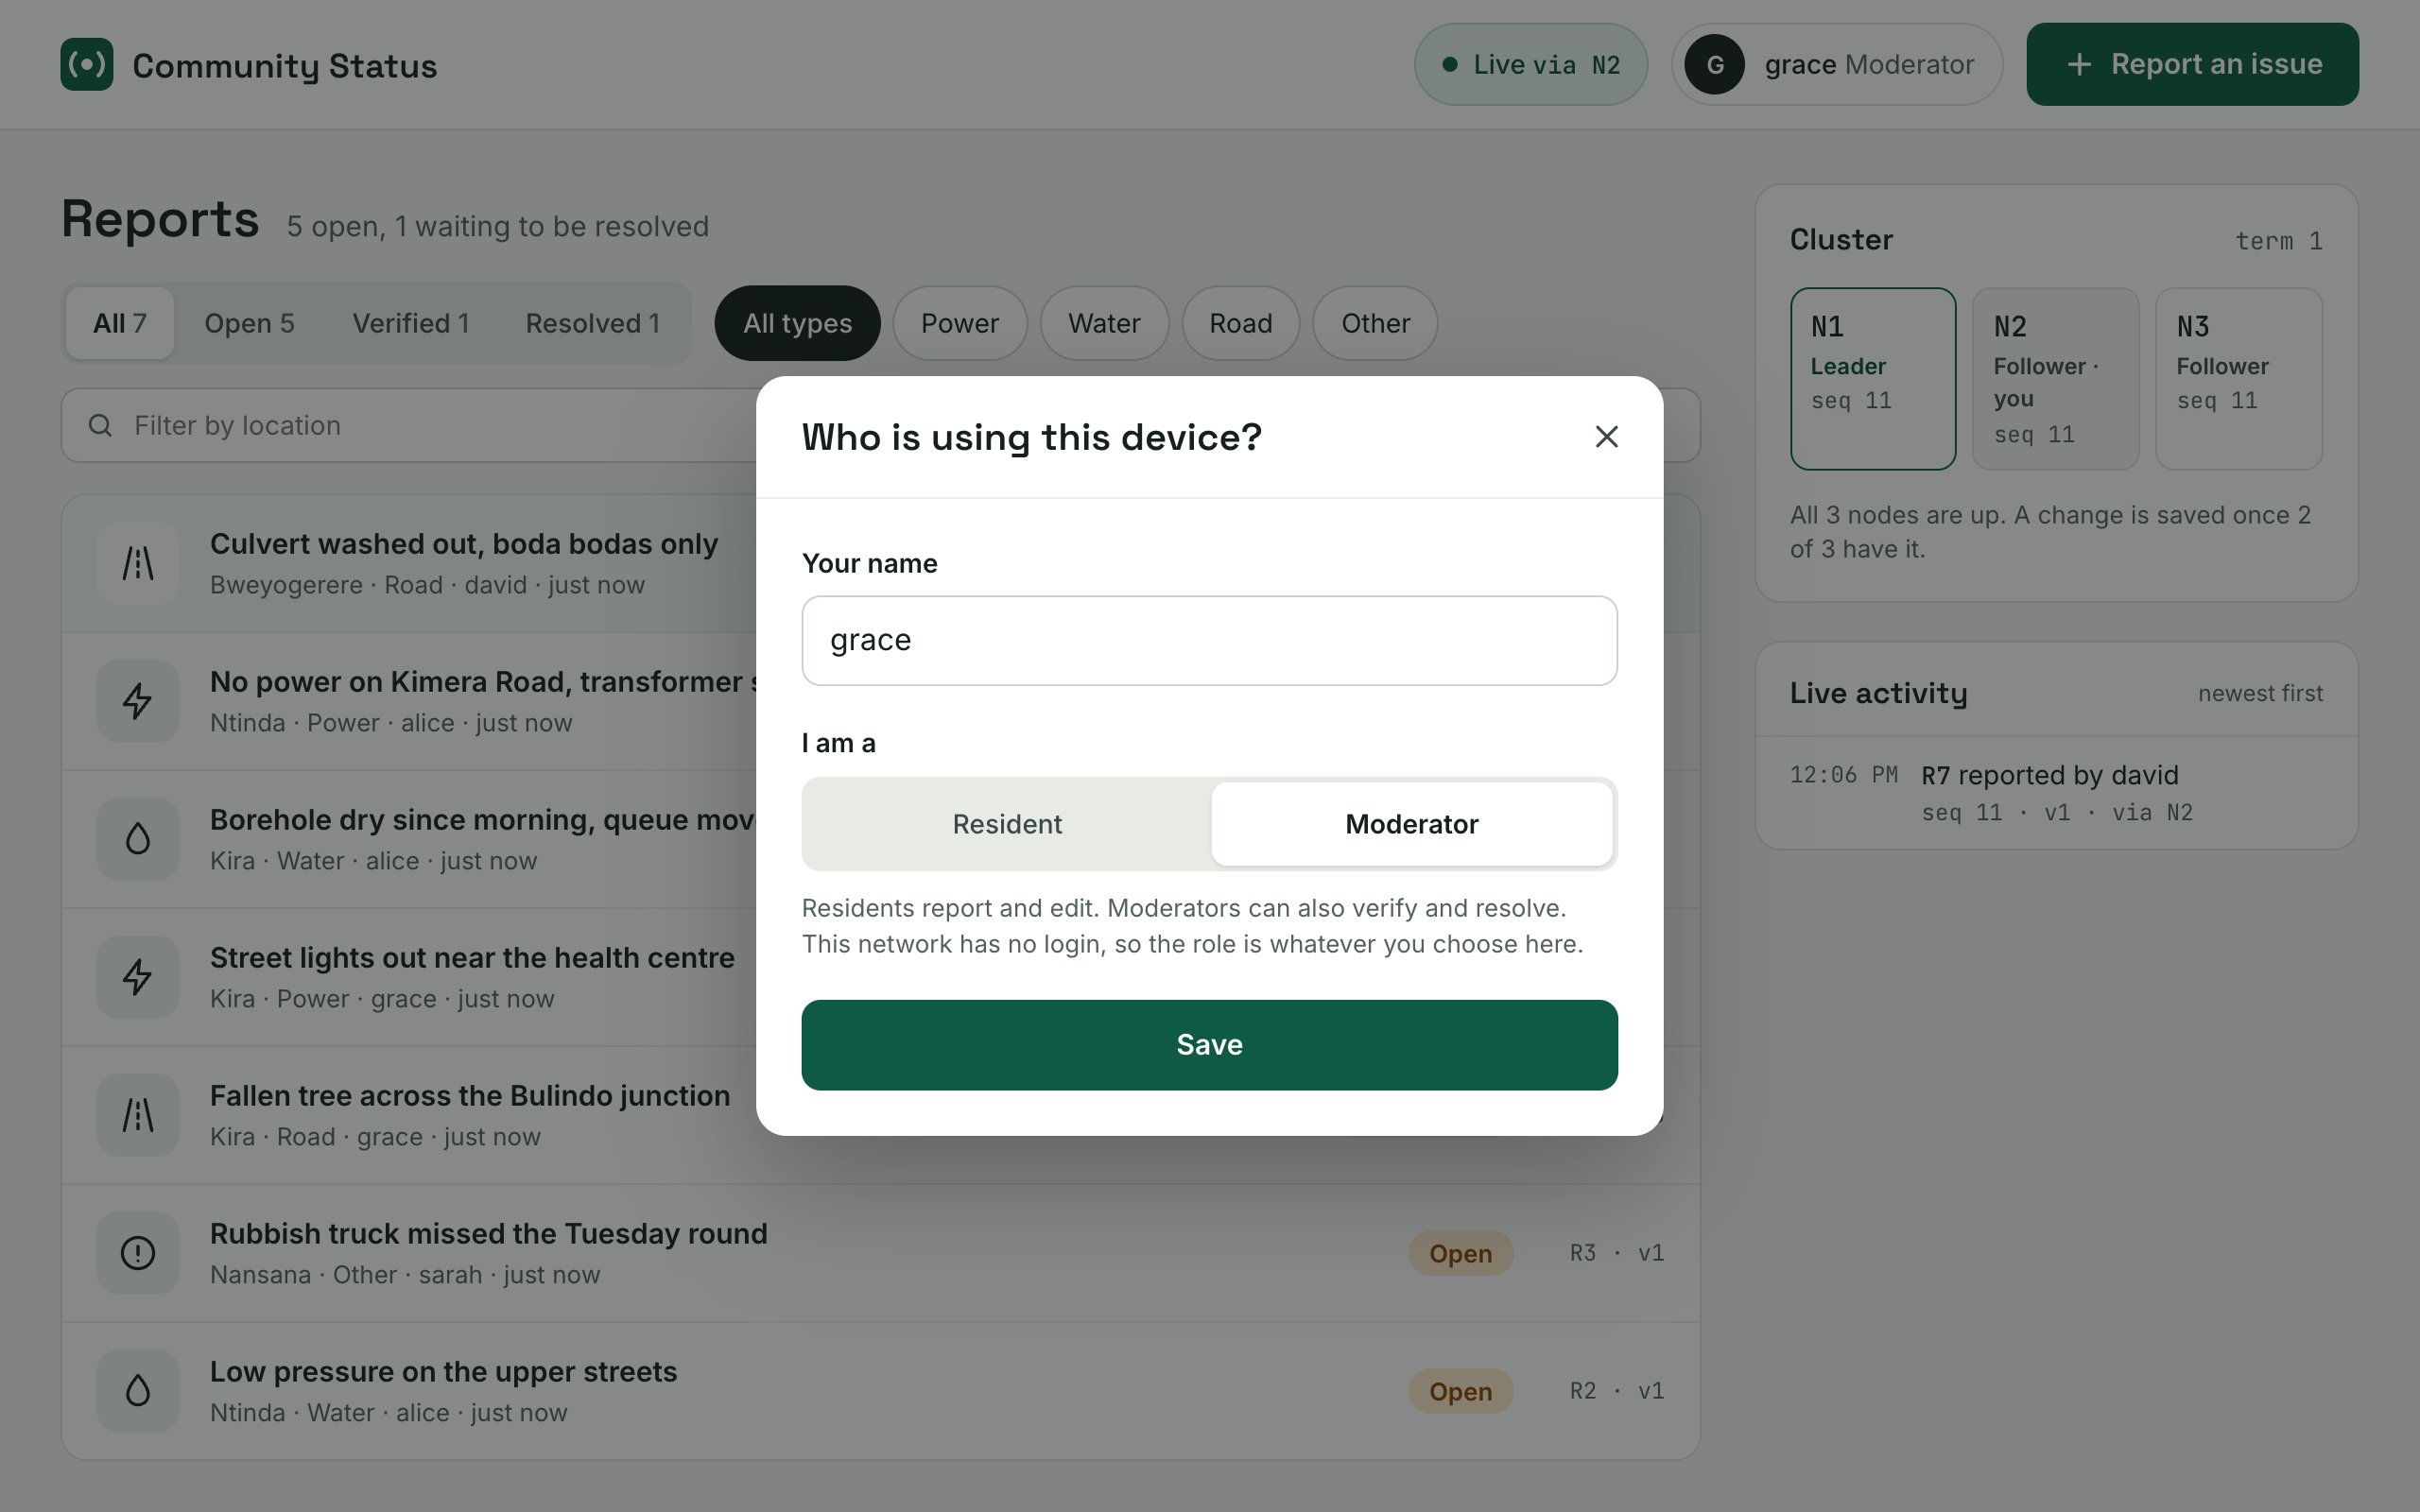
\includegraphics[width=0.8\textwidth]{guide-who.png}
\caption{Setting your name and role.}
\end{figure}

\subsection{Reporting a problem}

\begin{enumerate}
\item Press \ui{Report an issue}.
\item Pick the kind of problem: Power, Water, Road or Other.
\item Say where it is and describe it in a sentence or two.
\item Check your name and press \ui{Post report}.
\end{enumerate}
The report appears at the top of the list on every screen, marked \ui{Open}.

\begin{figure}[H]
\centering
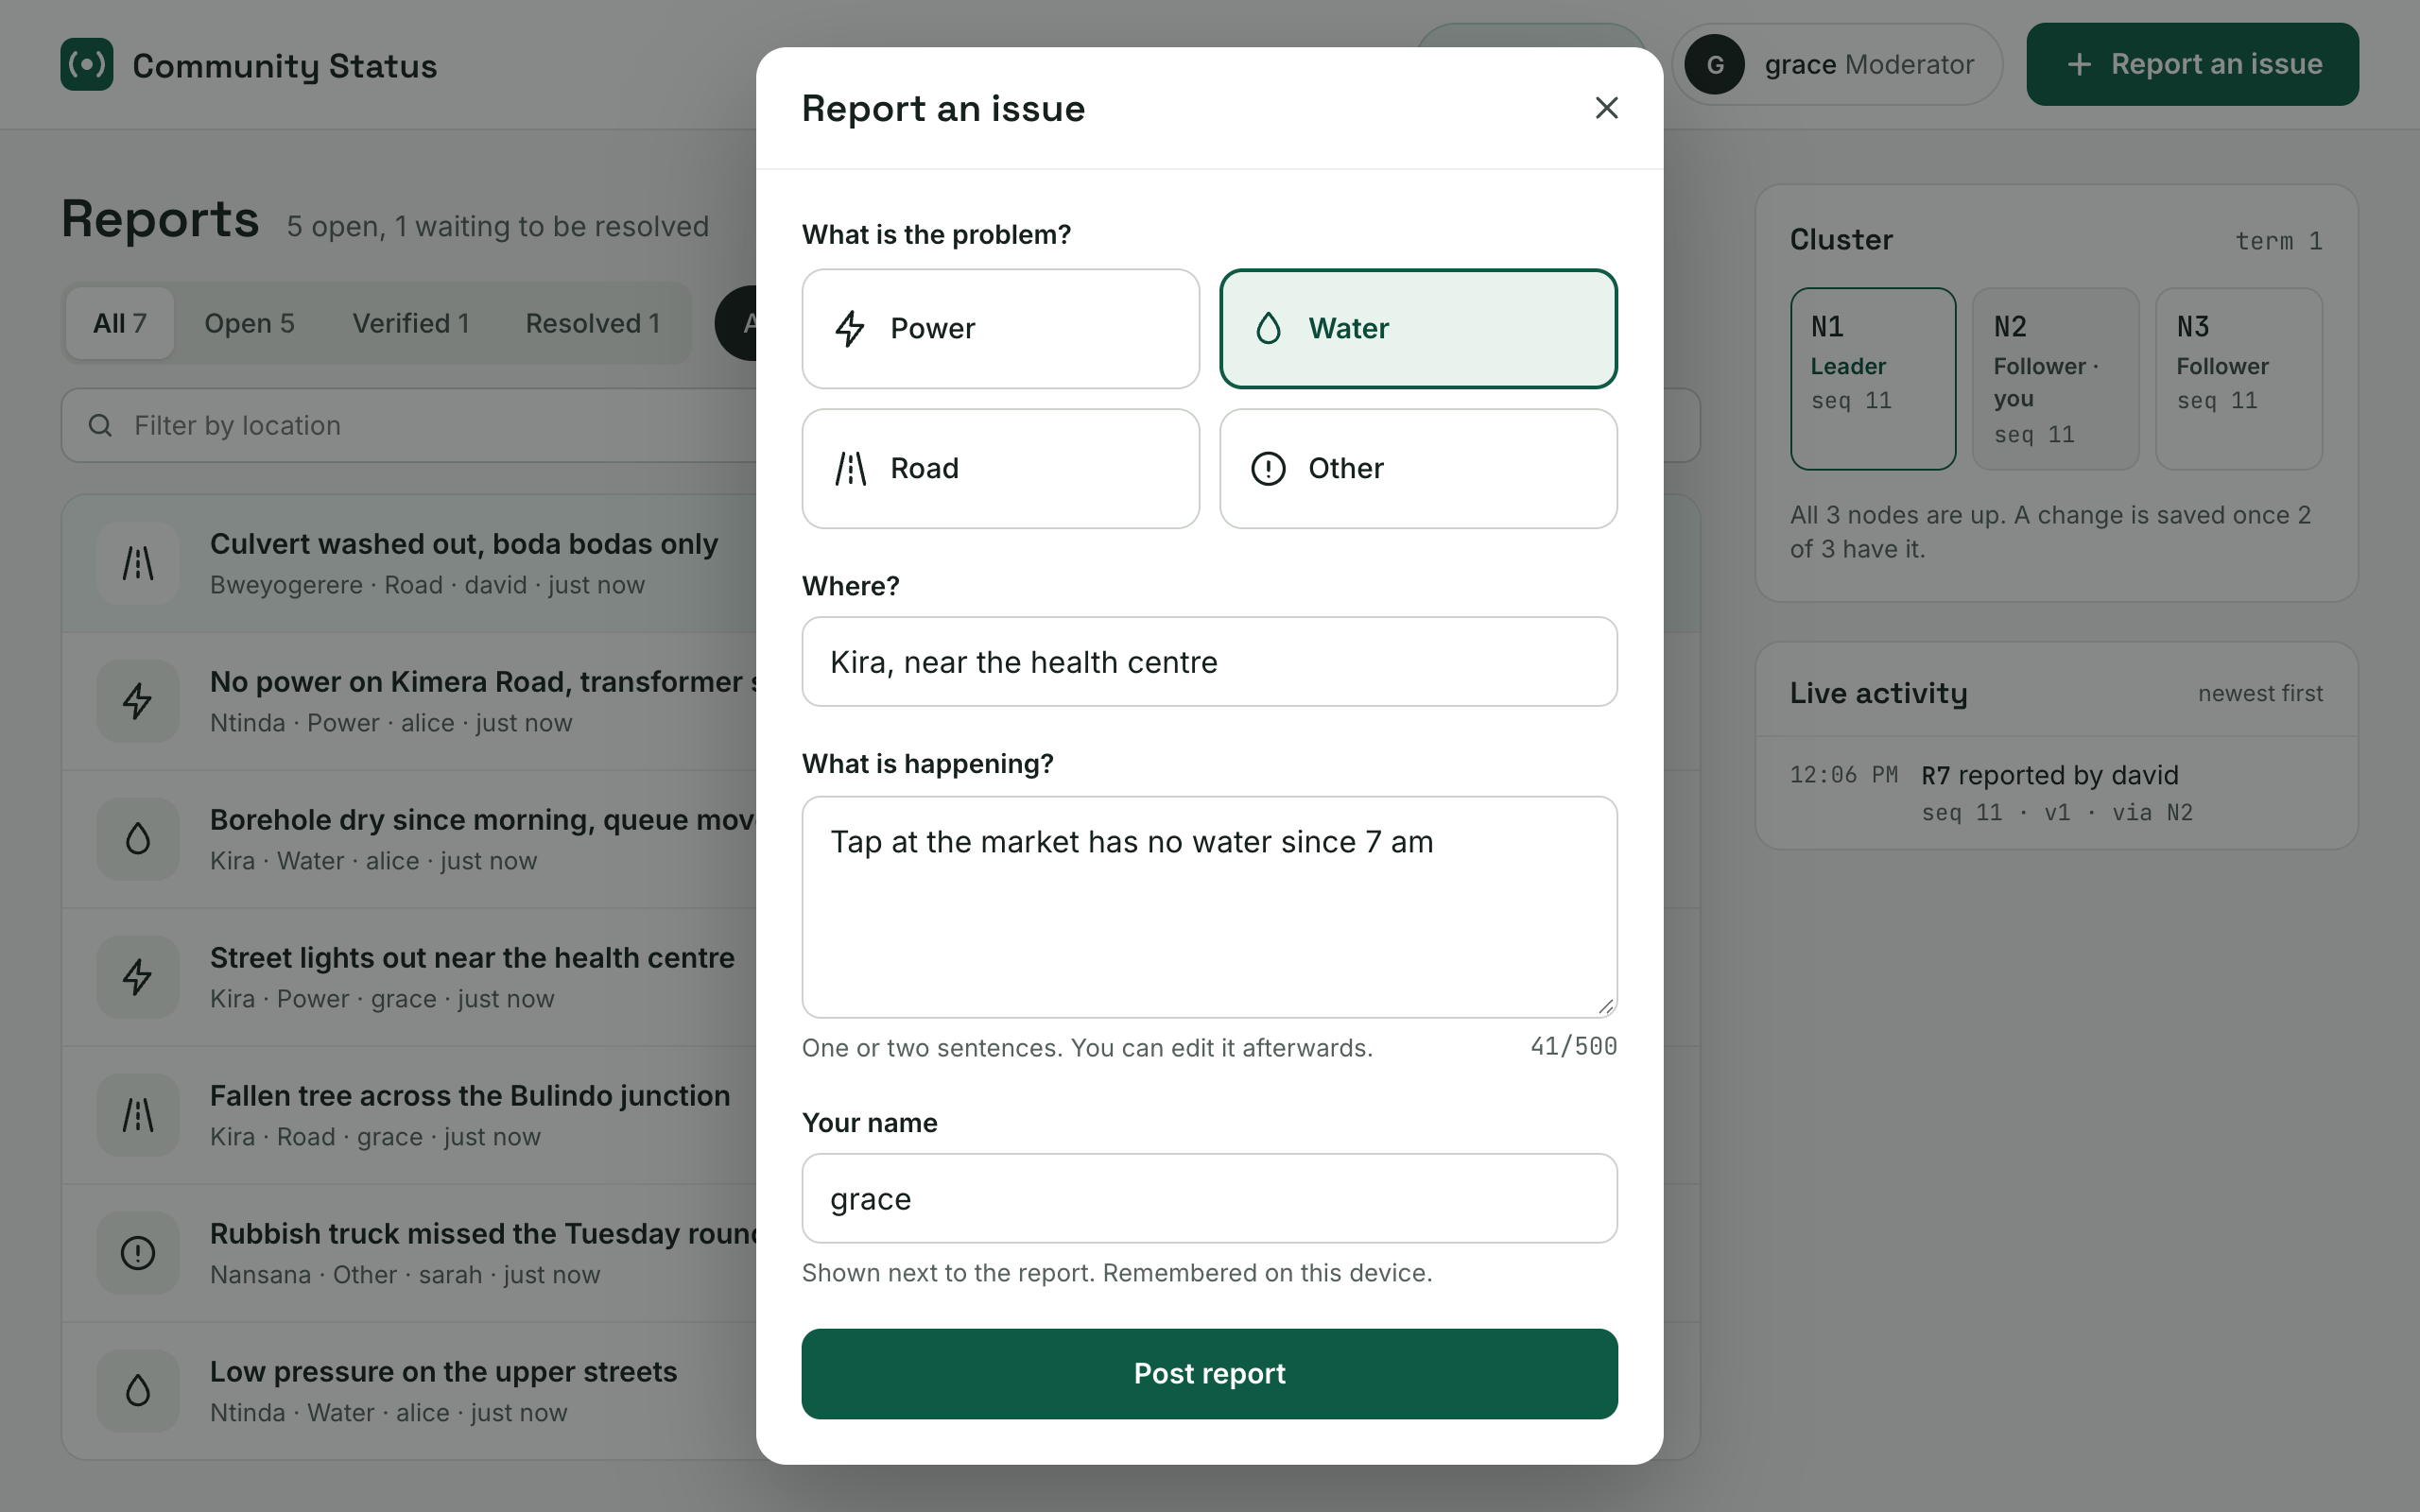
\includegraphics[width=0.8\textwidth]{guide-submit.png}
\caption{Reporting a problem: pick the kind, say where, describe it, and post.}
\end{figure}

\subsection{Finding reports}

\begin{itemize}
\item The tabs \ui{All}, \ui{Open}, \ui{Verified} and \ui{Resolved} filter by state. The number on
each tab is how many reports it holds.
\item The buttons \ui{Power}, \ui{Water}, \ui{Road} and \ui{Other} filter by kind.
\item Typing in \ui{Filter by location} keeps only the reports whose location contains what you
typed.
\end{itemize}
The most recently changed report is always at the top. A report that changed in the last few
seconds is highlighted and labelled \ui{Just updated}.

\subsection{Looking at one report}

Click a report. A panel opens showing its full text, where it is in the journey
Open~$\rightarrow$~Verified~$\rightarrow$~Resolved, and its \ui{History}: every change ever made
to it, who made it and when.

\begin{figure}[H]
\centering
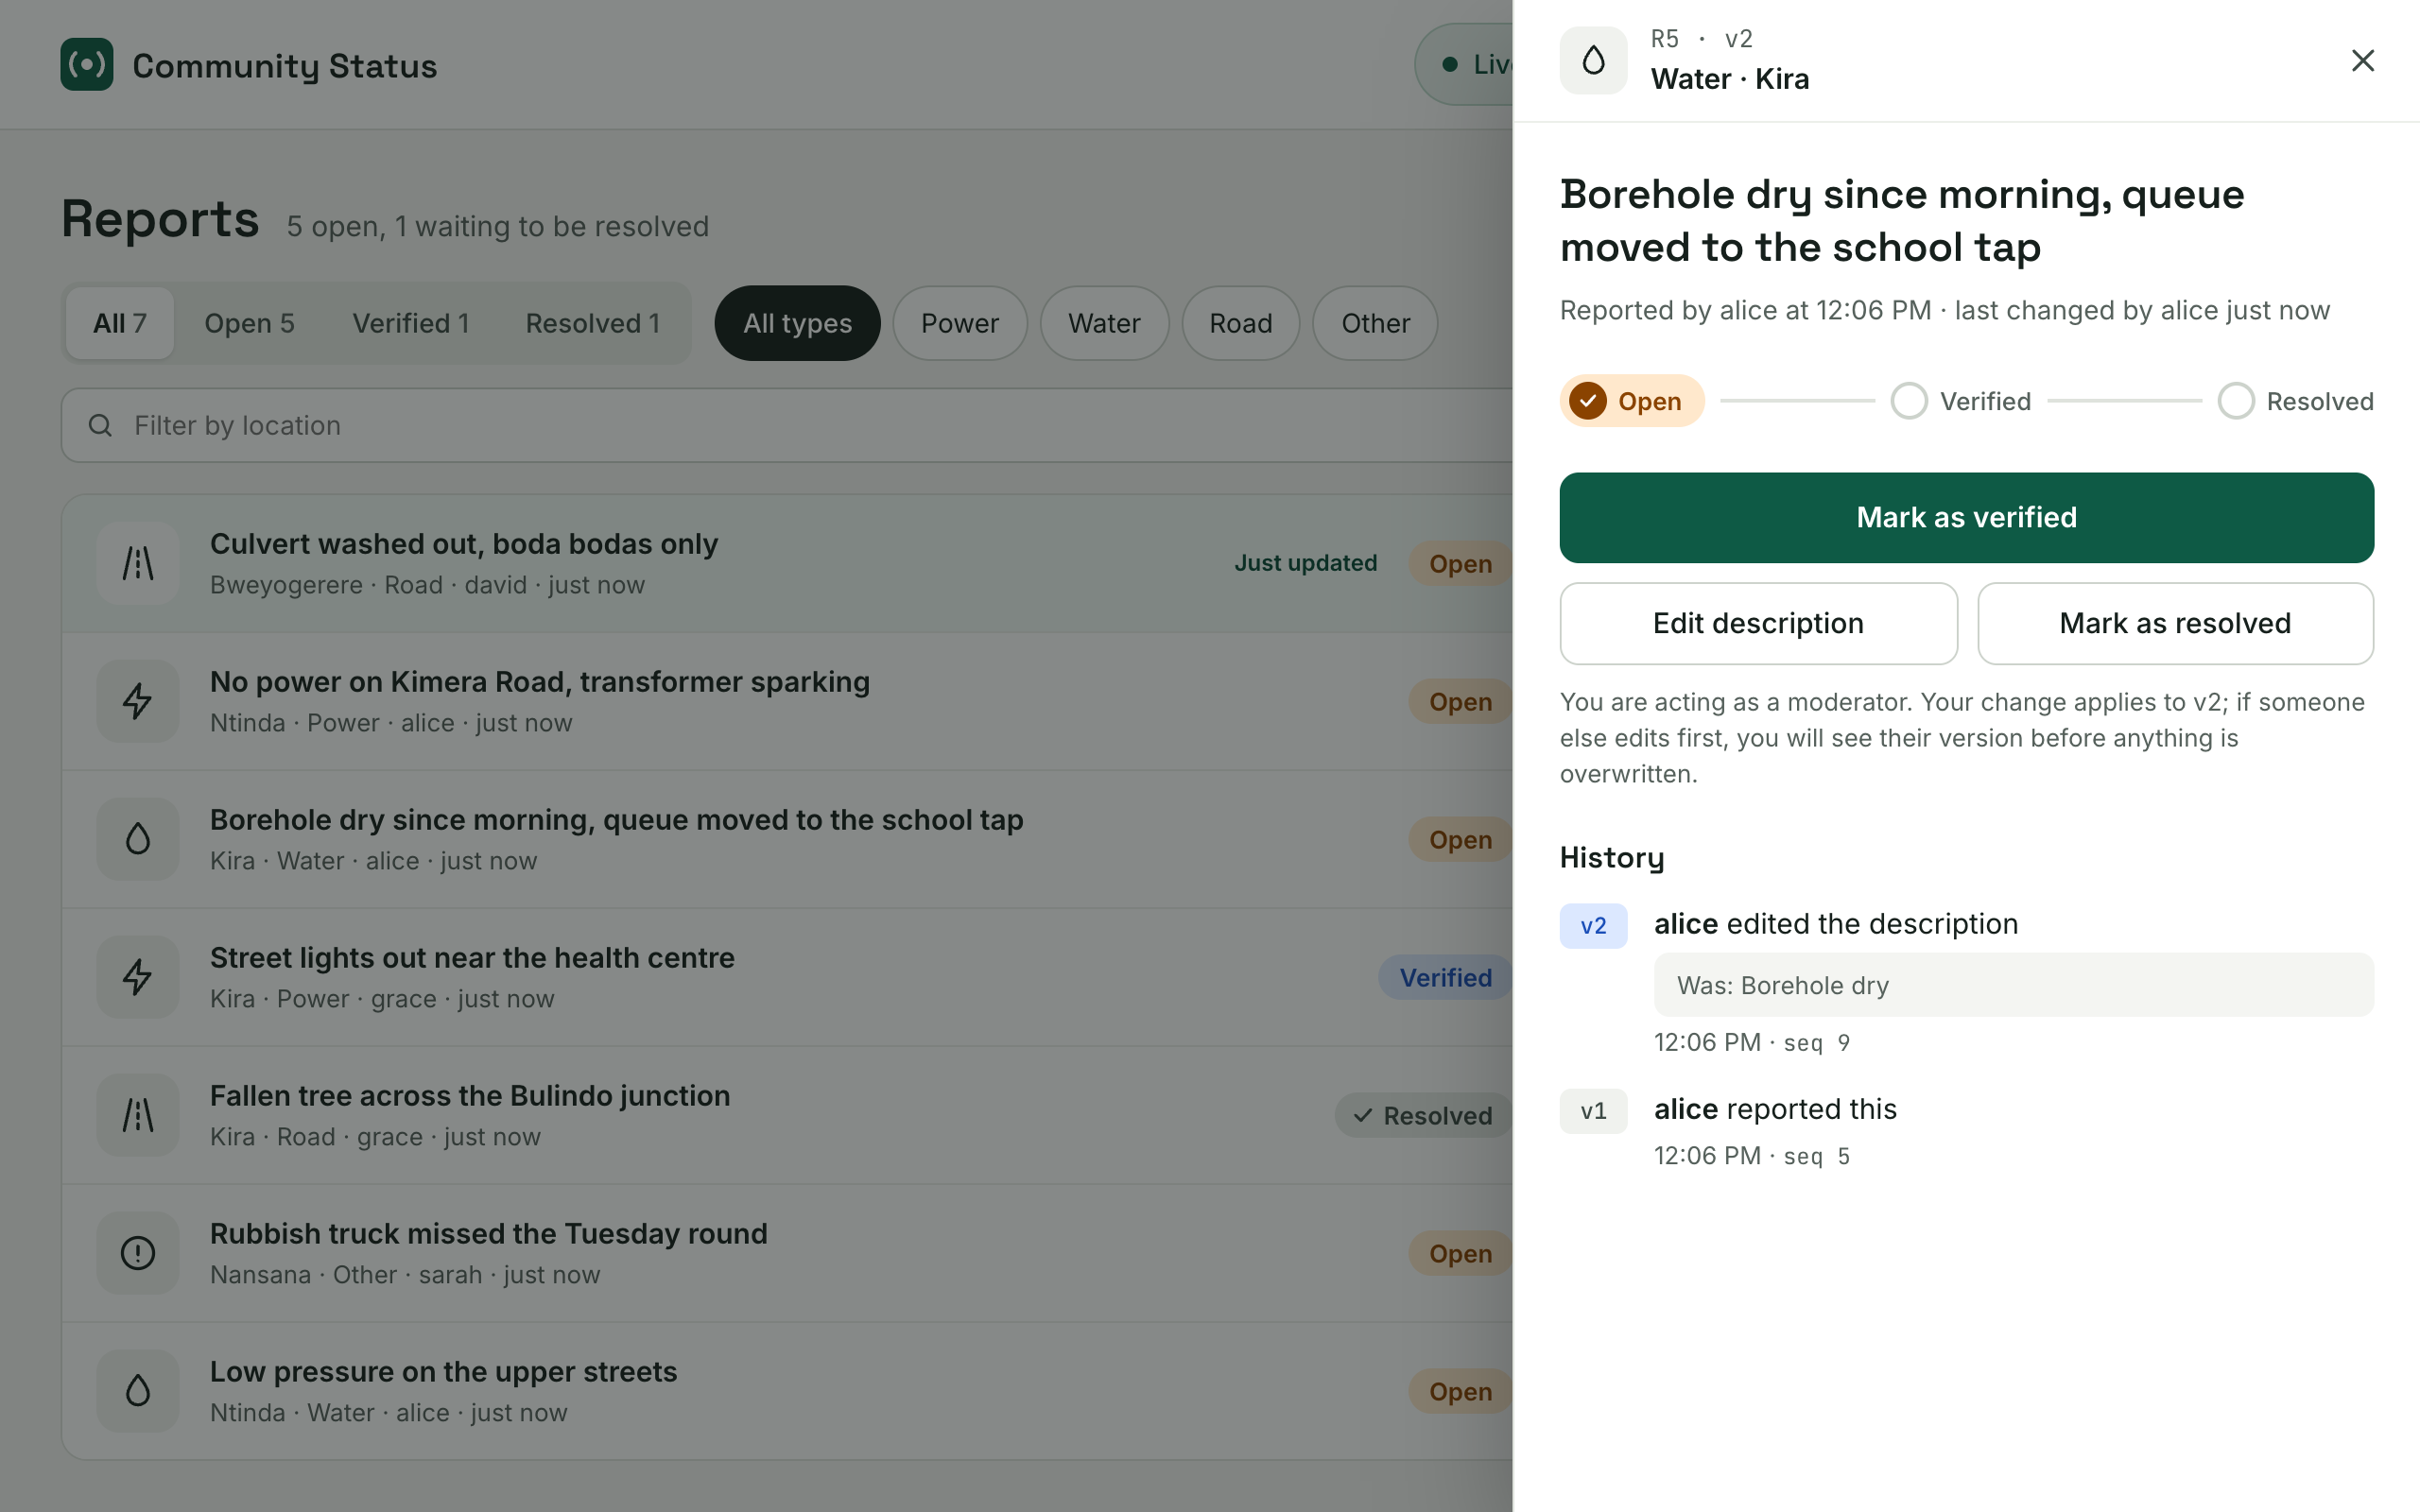
\includegraphics[width=0.9\textwidth]{guide-detail.png}
\caption{One report opened. The panel on the right shows its state, the actions a moderator can take, and its history.}
\end{figure}

\subsection{Editing, verifying and resolving}

In the report panel:
\begin{itemize}
\item \ui{Edit description} lets anyone correct the wording.
\item Moderators also see \ui{Mark as verified}, \ui{Mark as resolved} and \ui{Reopen}.
\end{itemize}

\subsection{When someone else changed the report first}

If another person saved a change to the same report while you were working on yours, a box
appears titled \emph{``This report changed while you were editing''}. It shows the latest version
and your unsaved change side by side. You choose one of two buttons:
\begin{itemize}
\item \ui{Apply my edit to the latest version} saves your change on top of theirs.
\item \ui{Discard my edit} drops your change and keeps theirs.
\end{itemize}

\begin{figure}[H]
\centering
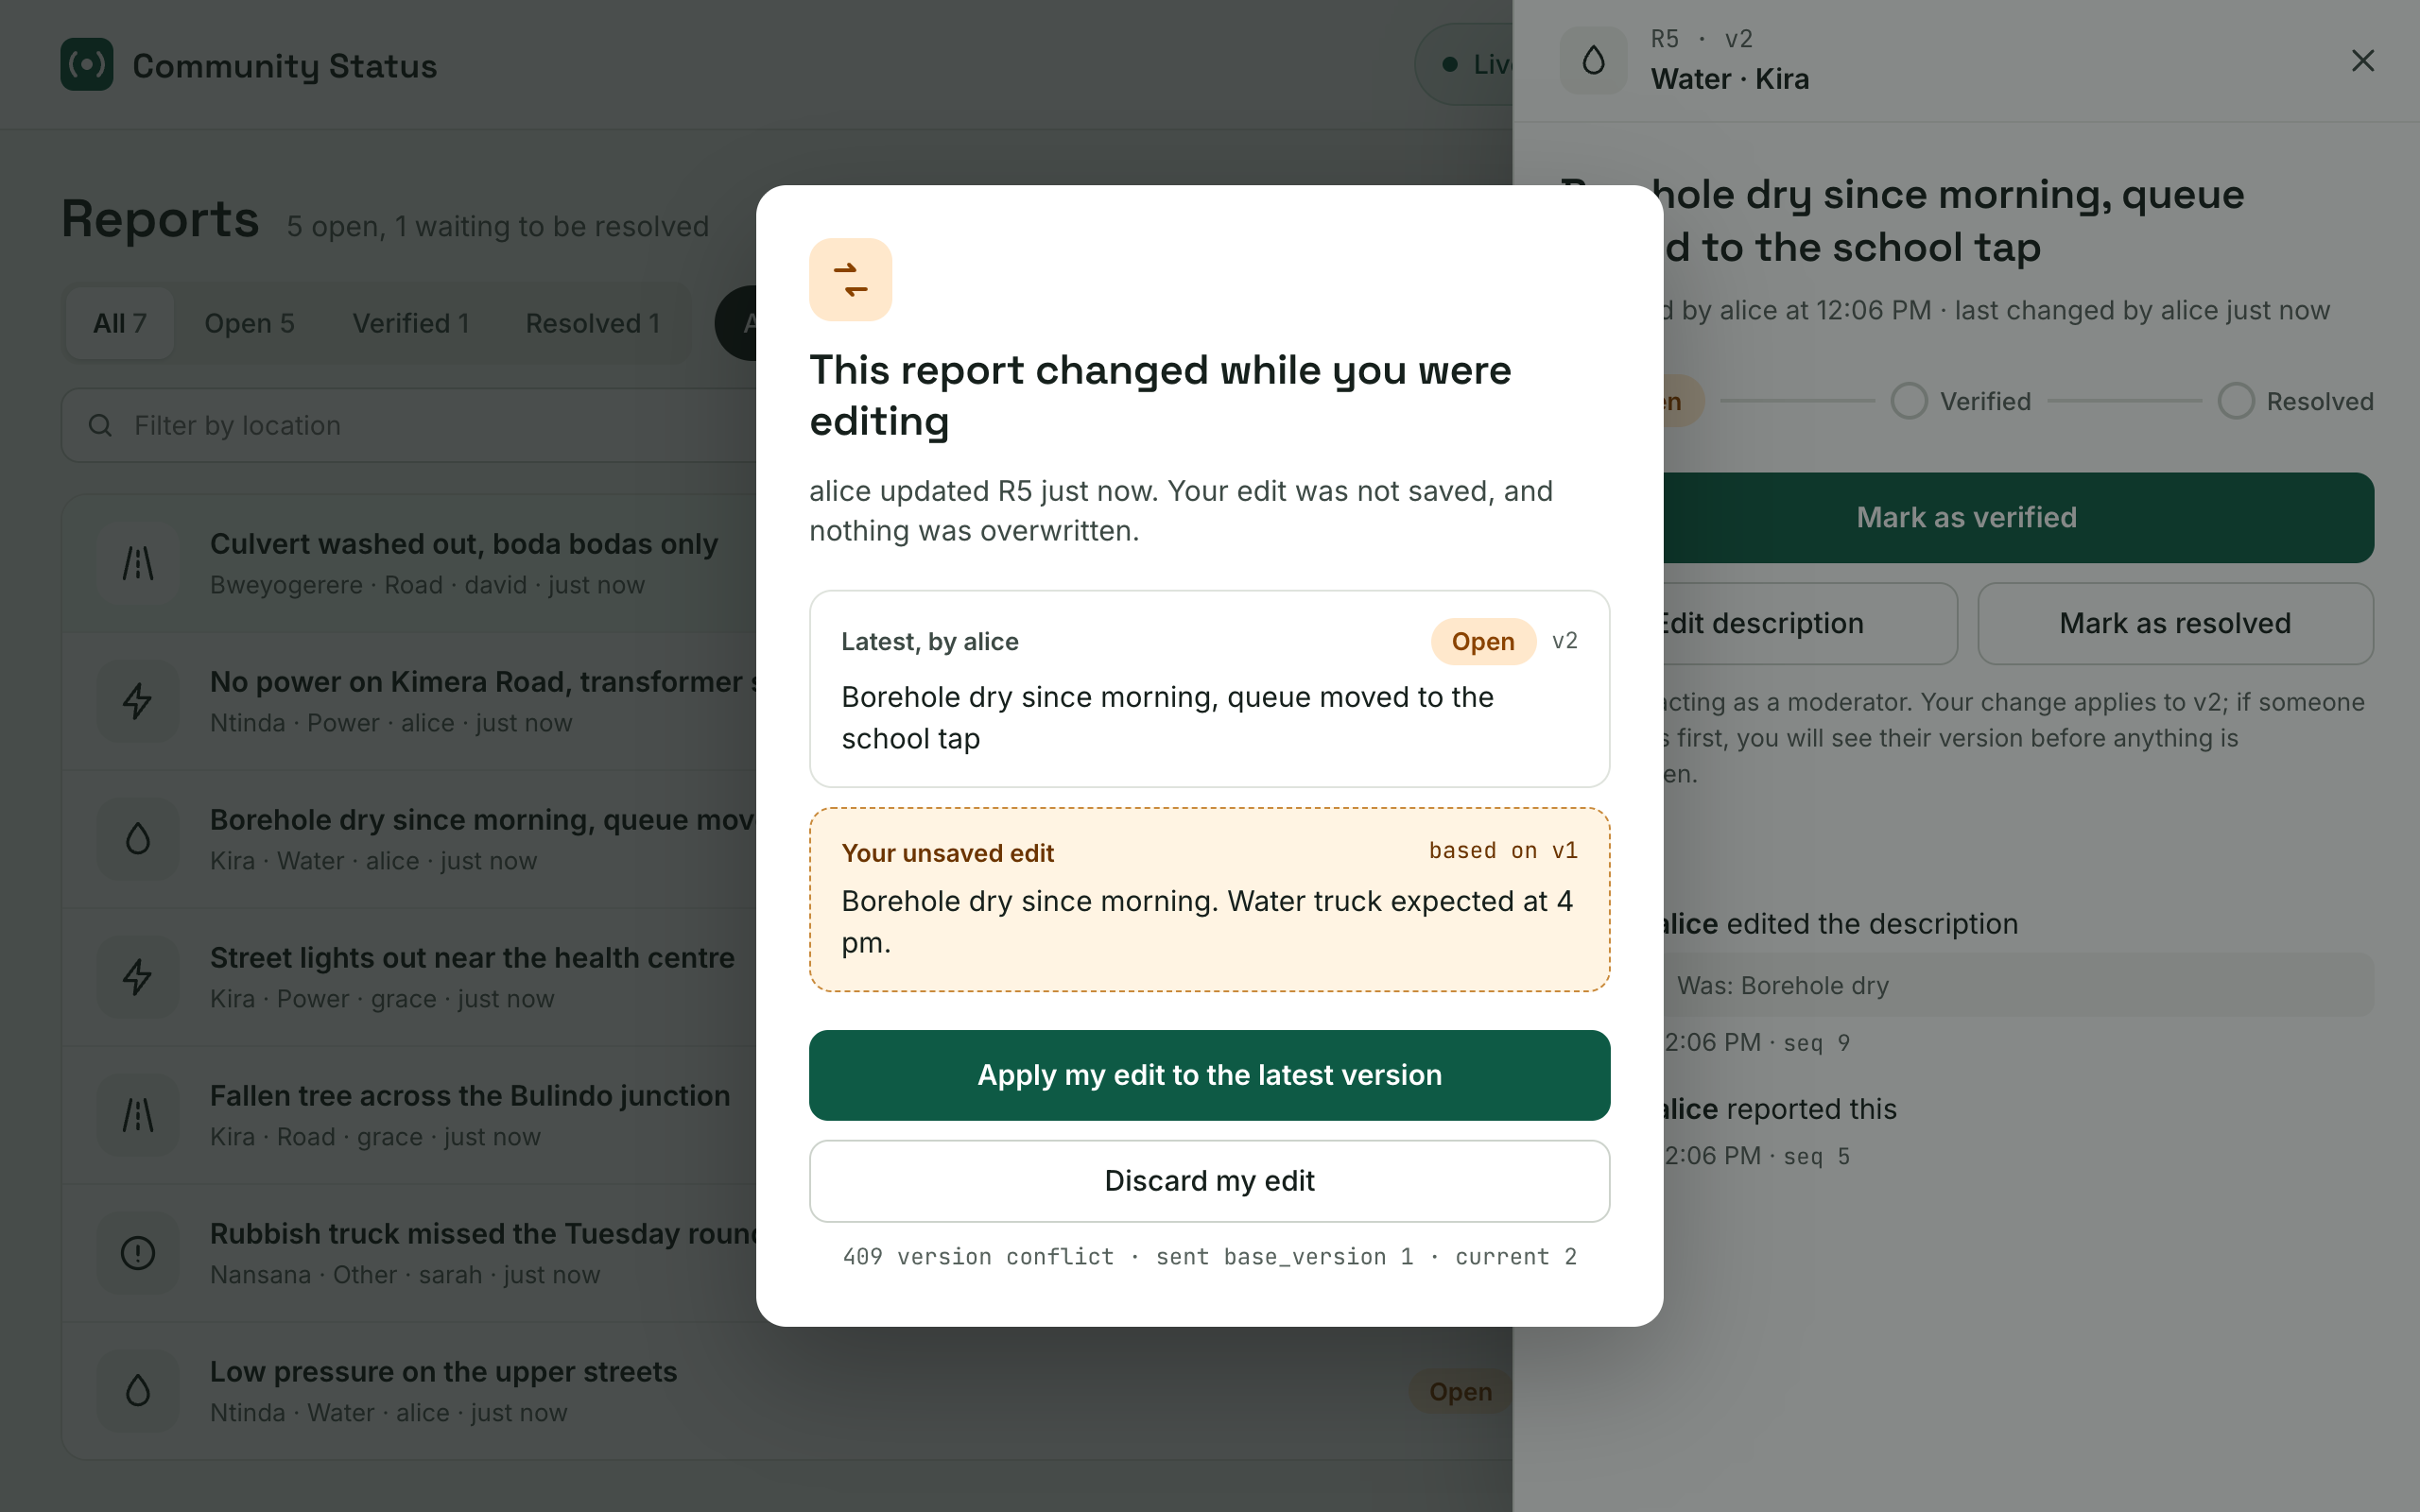
\includegraphics[width=0.9\textwidth]{guide-conflict.png}
\caption{Two people changed the same report. The latest version is shown above your unsaved change, and you choose what happens.}
\end{figure}

\subsection{Reading the cluster card}

The \ui{Cluster} box on the right shows the three nodes. For each one you can see whether it is
the \ui{Leader}, a \ui{Follower} or \ui{Down}, which one your browser is connected to
(marked ``you''), and a number called \texttt{seq}, which counts how many changes that node has
recorded. If the three numbers are equal, all three copies are identical. A sentence underneath
explains in words what currently works.

The \ui{Live activity} box below it lists changes as they happen, newest first.

\subsection{On a phone}

The same address works on a phone. The layout rearranges itself and the \ui{Report an issue}
button stays at the bottom of the screen.

\begin{figure}[H]
\centering
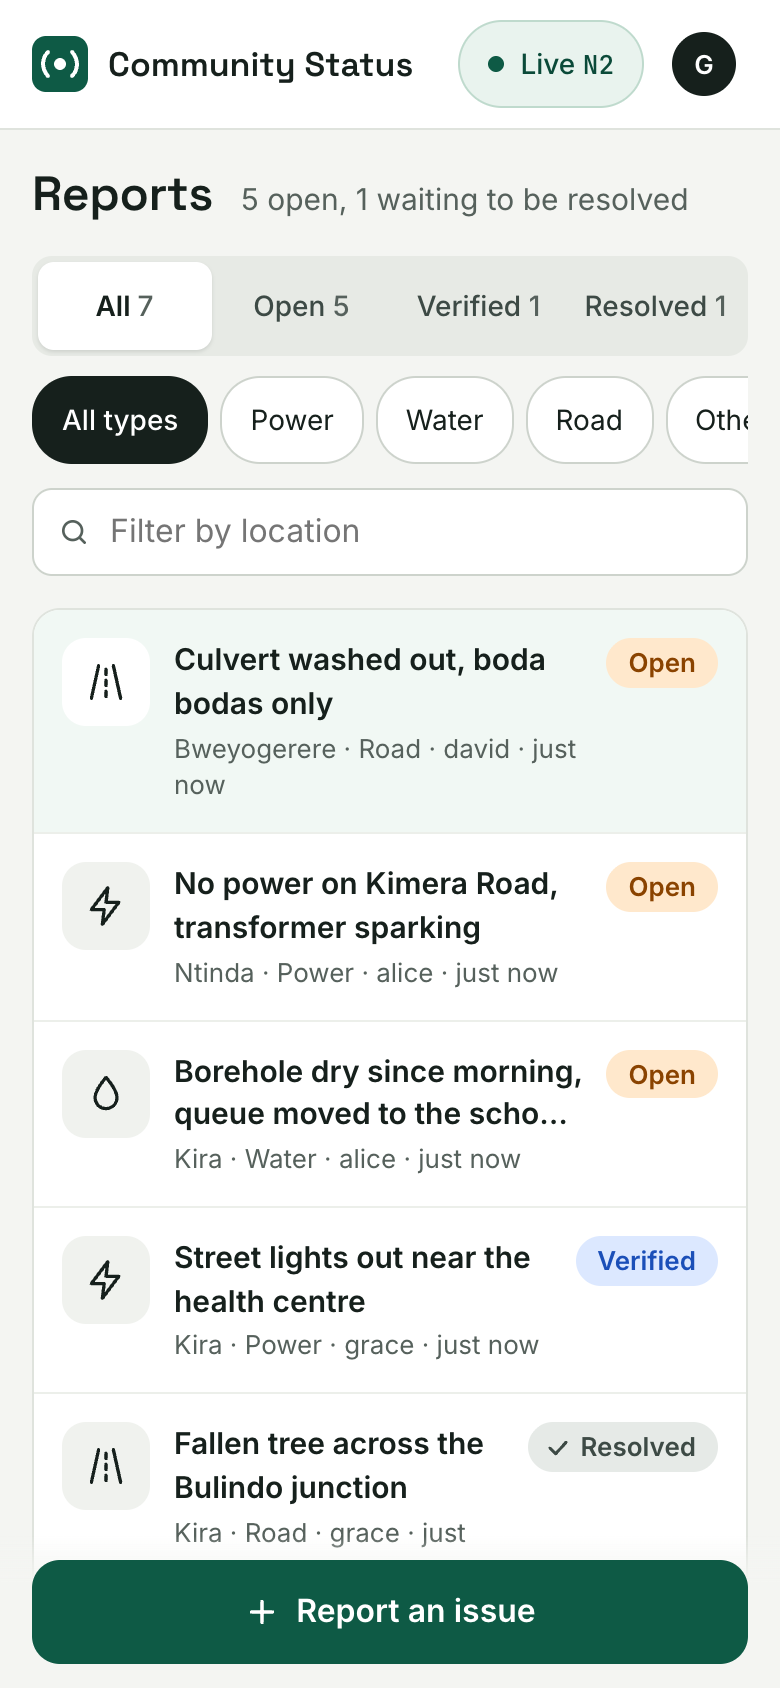
\includegraphics[height=0.42\textheight]{guide-mobile.png}\hspace{1cm}
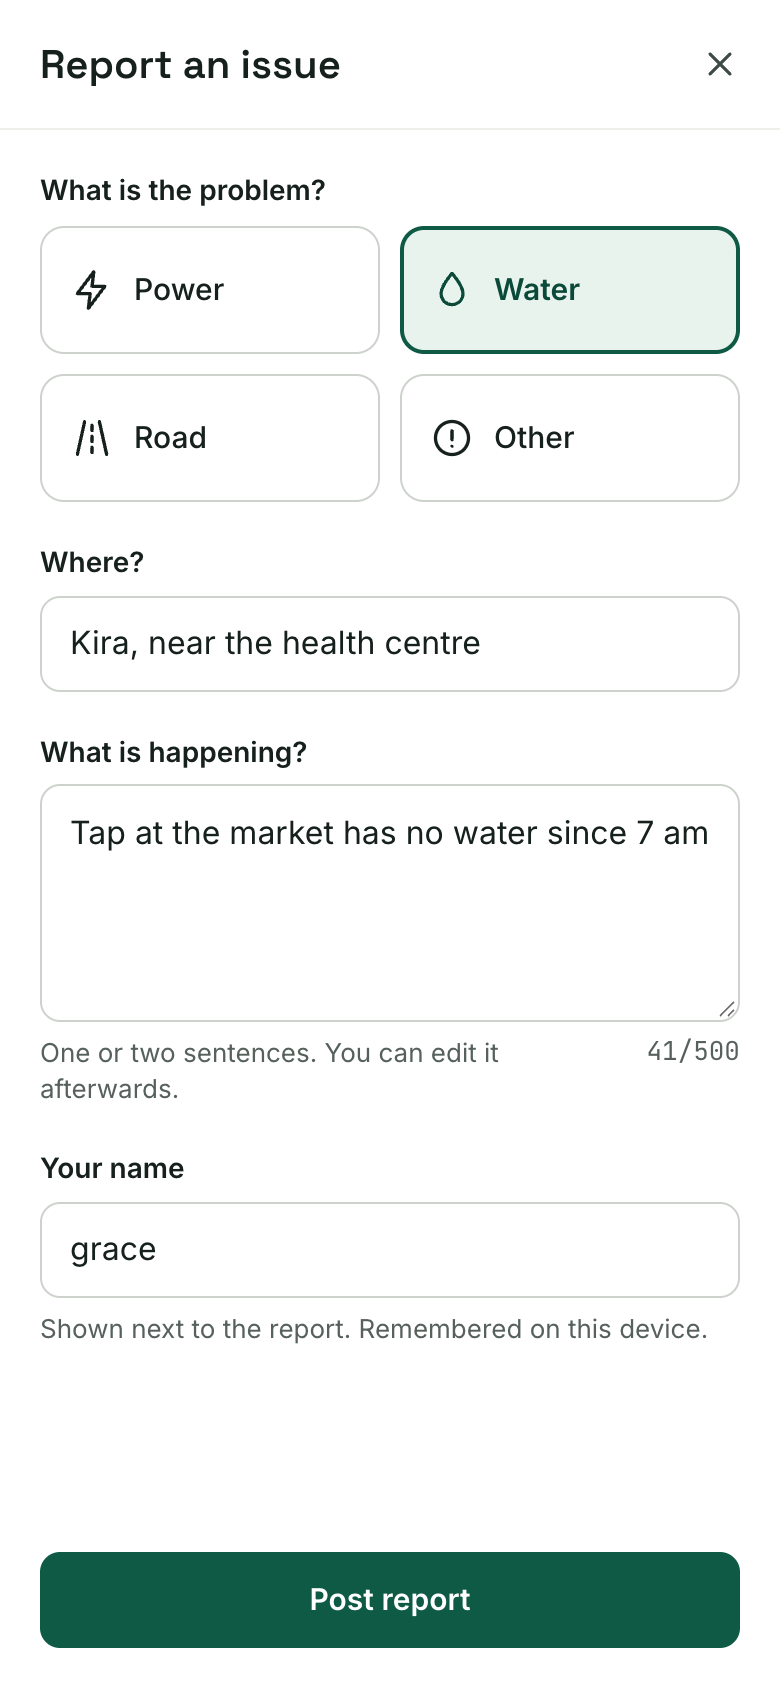
\includegraphics[height=0.42\textheight]{guide-mobile-submit.png}
\caption{The list and the report form on a phone-sized screen.}
\end{figure}

\subsection{Using the command line instead}

Everything the web app does can also be done from a terminal:
\begin{verbatim}
python3 -m csn.cli submit --type water --location Kira \
        --description "Borehole dry" --user alice
python3 -m csn.cli list
python3 -m csn.cli list --type water --status open
python3 -m csn.cli get R1
python3 -m csn.cli update R1 --user grace --role moderator \
        --base-version 1 --status verified
python3 -m csn.cli watch
\end{verbatim}
\texttt{-{}-base-version} is the version number you last saw (use \texttt{get} to see it).
\texttt{watch} prints every change as it happens until you press Ctrl-C.

\section{Try breaking it}

The best way to understand the system is to watch it survive a failure.

\begin{enumerate}
\item Start the three nodes by hand (three terminals) and open
\texttt{http://127.0.0.1:8002/} in a browser. Post one or two reports.
\item Look at the \ui{Cluster} box: N1 is the leader.
\item Go to the terminal running N1 and press Ctrl-C to kill it.
\item Watch the browser. Within about three seconds N1 shows as \ui{Down} and N2 becomes the
\ui{Leader}. The note under the cards says everything keeps working on 2 of 3 nodes.
\item Post another report. It works.
\item Start N1 again with \texttt{python3 -m csn.server -{}-id N1}. It comes back as a follower
and its \texttt{seq} number catches up with the others in a fraction of a second.
\item Now kill the node your browser is connected to (N2). A dark banner appears saying the page
reconnected through another node and that you missed nothing.
\end{enumerate}

\begin{figure}[H]
\centering
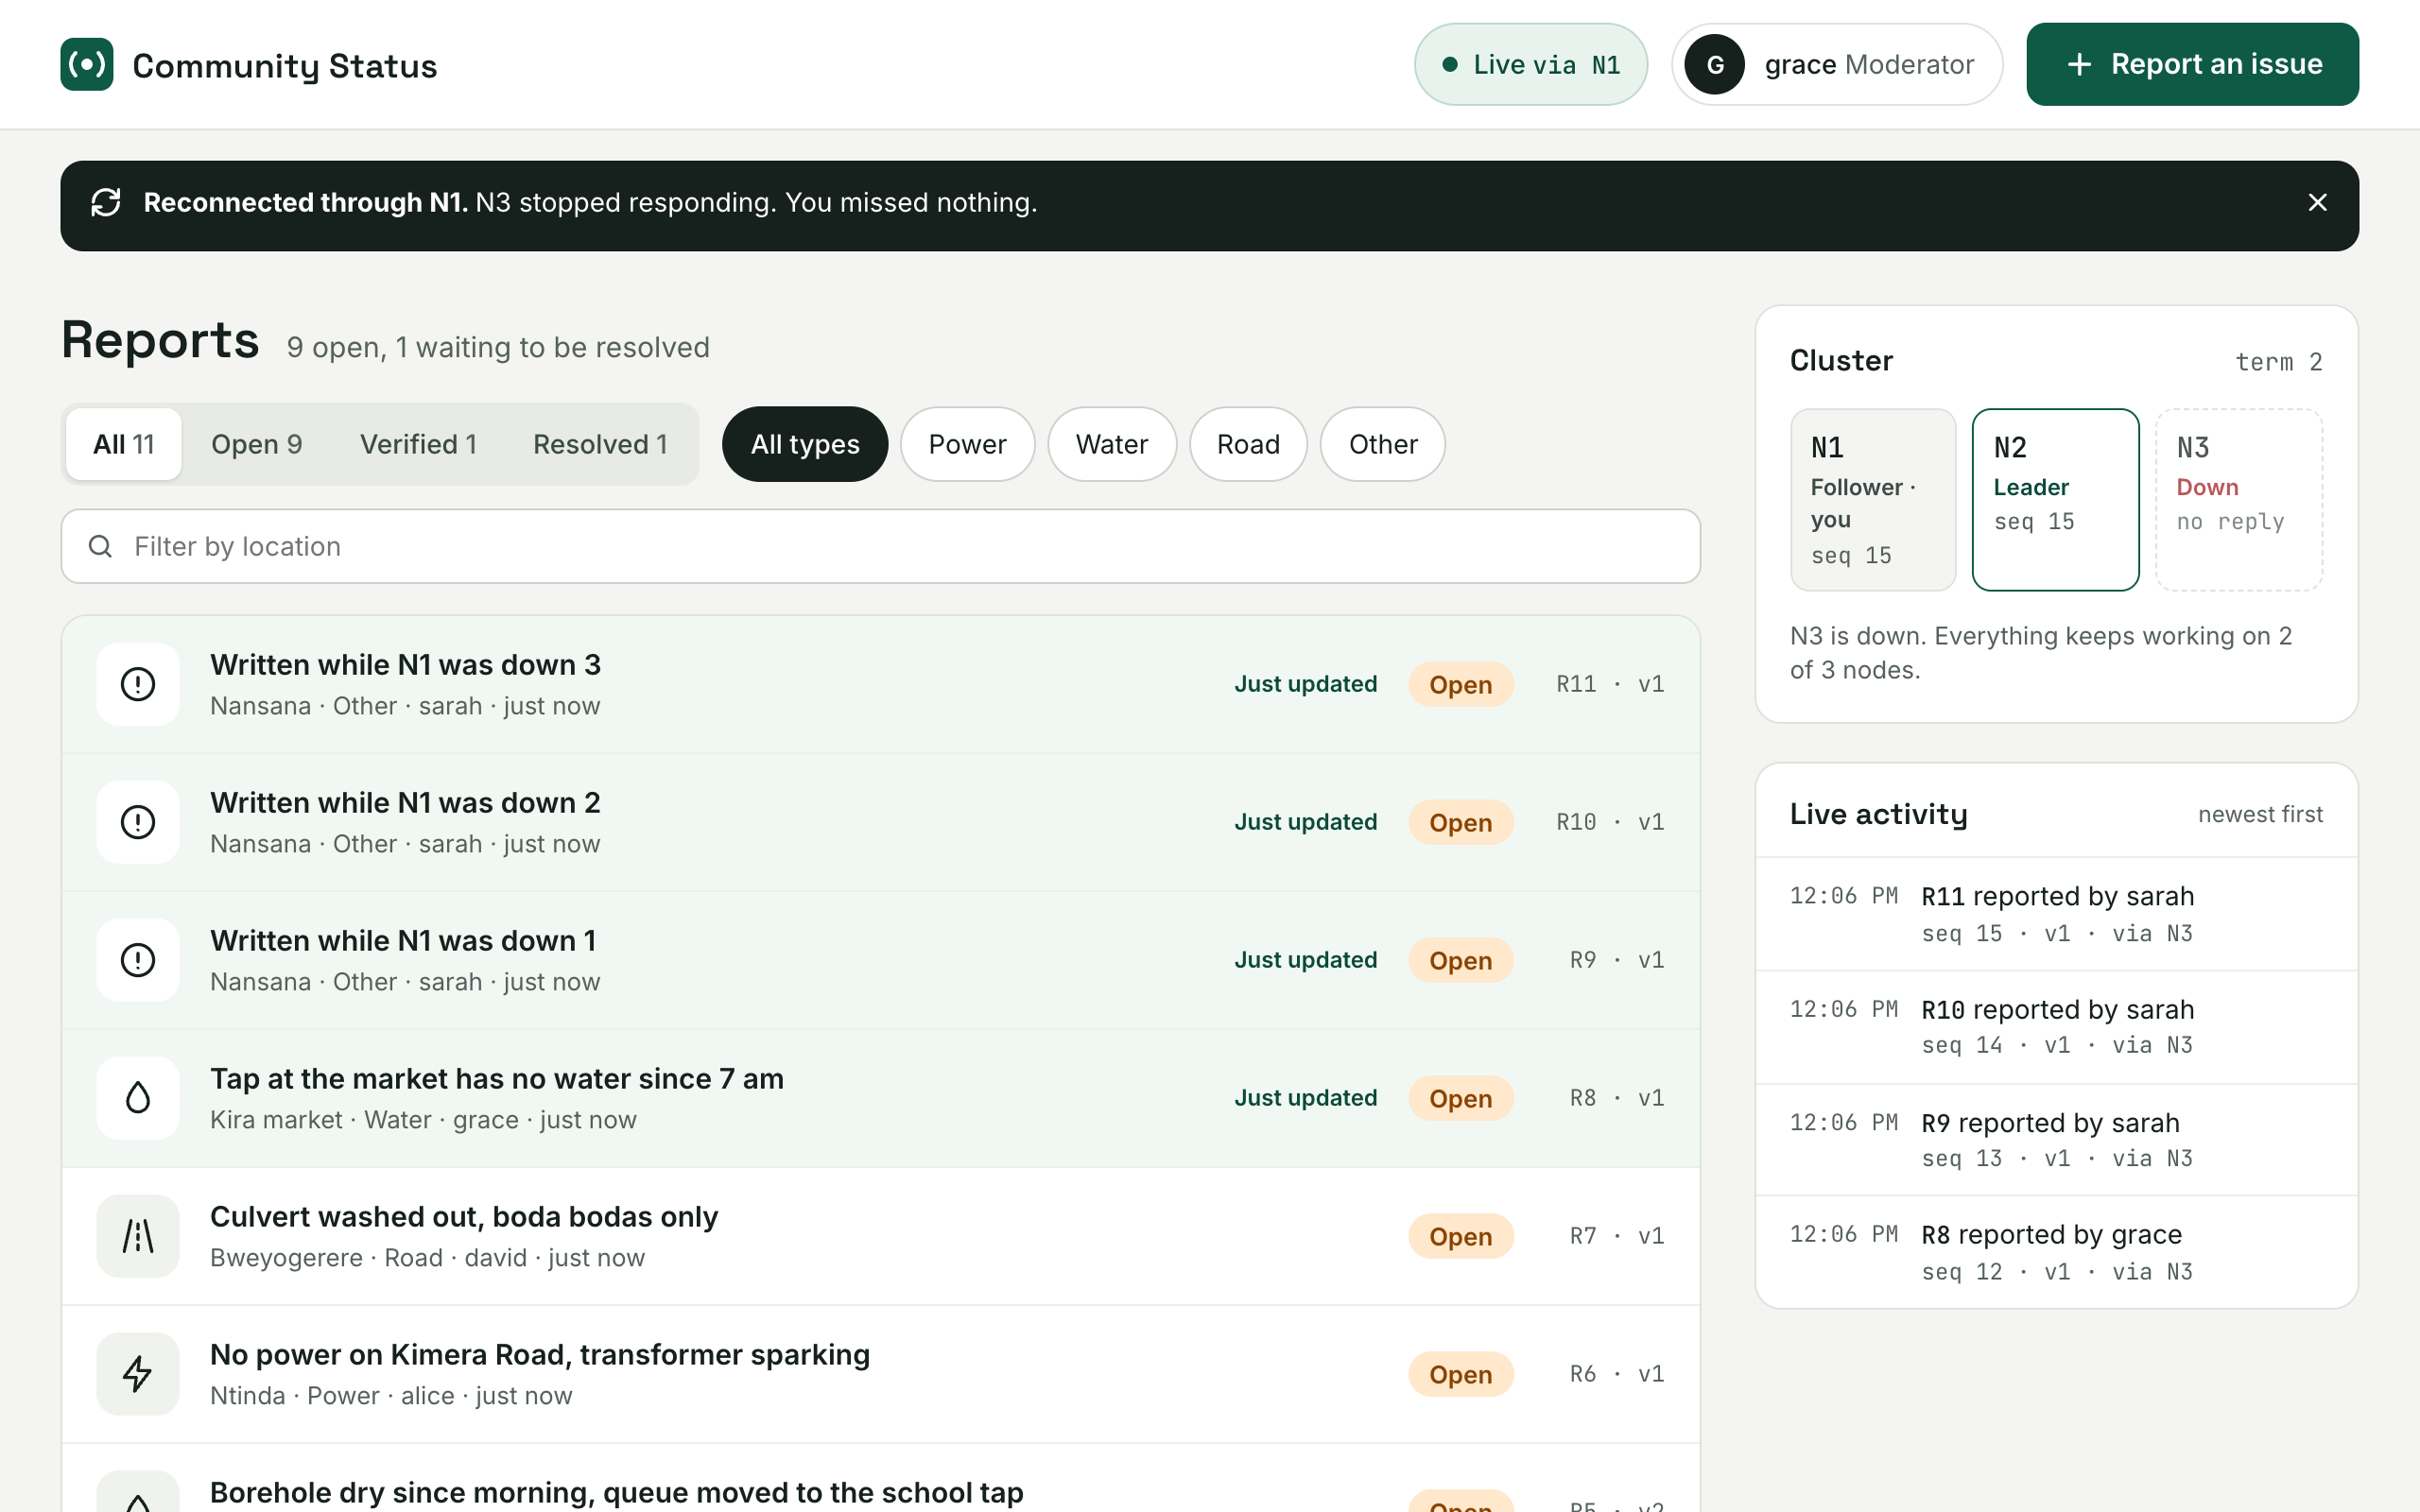
\includegraphics[width=0.95\textwidth]{guide-failover.png}
\caption{The node this browser was connected to (N3) was killed. The page moved to N1 by itself, the banner says so, and the cluster box shows N3 as down while everything keeps working.}
\end{figure}

\section{What it cannot do}
\label{sec:limits}

This is a learning prototype, and it is honest about its limits.

\begin{itemize}
\item \textbf{It survives one dead computer, not two.} With two of three down, reports can be
read but not changed.
\item \textbf{There are no accounts or passwords.} Anyone can type any name and choose the
moderator role. A real deployment would need proper sign-in.
\item \textbf{There is a pause of about three seconds} for changes when the leader dies. Reading
continues throughout.
\item \textbf{A follower can be a split second behind.} If you read from the one follower that
has not yet received the newest change, you may briefly see the previous version.
\item \textbf{A broken network between nodes is handled only partly.} If the leader is cut off
from the others but still running, it cannot save anything (it has no majority) and steps down
when the connection returns, but for a moment people connected to it may see changes that were
never truly saved.
\item \textbf{The notebook grows forever.} Old entries are never cleaned up, which is fine for a
demonstration but not for years of use.
\end{itemize}

\section{If something goes wrong}

\begin{tabular}{@{}p{0.38\textwidth}p{0.57\textwidth}@{}}
\toprule
What you see & What to do \\
\midrule
``Address already in use'' when starting a node & Another copy is already running, or another
program uses port 8001, 8002 or 8003. Stop it and try again. \\
The page says ``Reconnecting\dots'' and never recovers & No node is running. Start them. \\
``Only 1 of 3 nodes is up'' & Start a second node; changes will work again straight away. \\
You want to start with an empty board & Stop the nodes, delete the \texttt{data} folder, start
them again. \\
\bottomrule
\end{tabular}

\section{Glossary}

\begin{description}[leftmargin=3.2cm,style=sameline]
\item[Node] One of the three programs that together make up the system.
\item[Leader] The node currently in charge of ordering changes.
\item[Follower] A node that copies what the leader does.
\item[Write-ahead log] The file in which a node writes every change before confirming it.
\item[Majority] More than half: here, two of the three nodes.
\item[Replication] Copying each change from the leader to the followers.
\item[Version] A counter on each report that goes up by one with every change.
\item[Conflict] Two people changing the same version of the same report.
\item[Heartbeat] The ``I am alive'' message nodes send each other every second.
\item[Failover] Switching to another node when one stops working.
\item[Live feed] The open connection through which a node pushes changes to a screen.
\end{description}

\end{document}
